% Created by tikzDevice version 0.12.3.1 on 2021-07-09 00:09:06
% !TEX encoding = UTF-8 Unicode
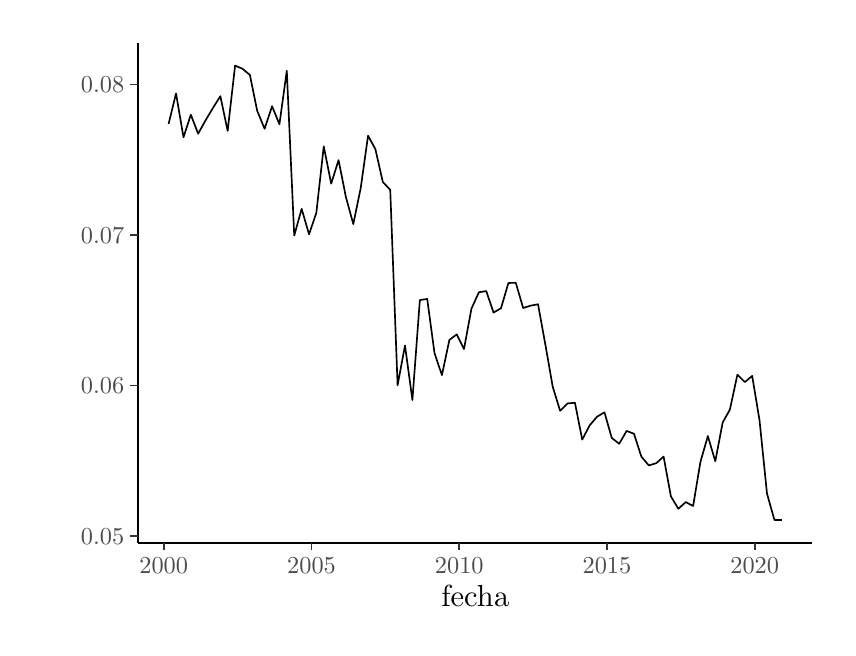
\begin{tikzpicture}[x=1pt,y=1pt]
\definecolor{fillColor}{RGB}{255,255,255}
\path[use as bounding box,fill=fillColor,fill opacity=0.00] (0,0) rectangle (289.08,216.81);
\begin{scope}
\path[clip] (  0.00,  0.00) rectangle (289.08,216.81);
\definecolor{drawColor}{RGB}{255,255,255}
\definecolor{fillColor}{RGB}{255,255,255}

\path[draw=drawColor,line width= 0.6pt,line join=round,line cap=round,fill=fillColor] (  0.00,  0.00) rectangle (289.08,216.81);
\end{scope}
\begin{scope}
\path[clip] ( 39.84, 30.69) rectangle (283.58,211.31);
\definecolor{fillColor}{RGB}{255,255,255}

\path[fill=fillColor] ( 39.84, 30.69) rectangle (283.58,211.31);
\definecolor{drawColor}{RGB}{0,0,0}

\path[draw=drawColor,line width= 0.6pt,line join=round] ( 50.92,182.03) --
	( 53.61,193.03) --
	( 56.30,177.20) --
	( 58.96,185.35) --
	( 61.59,178.50) --
	( 64.28,183.32) --
	( 66.97,187.83) --
	( 69.63,192.05) --
	( 72.26,179.51) --
	( 74.95,203.10) --
	( 77.64,201.95) --
	( 80.30,199.73) --
	( 82.93,186.78) --
	( 85.62,180.27) --
	( 88.31,188.44) --
	( 90.97,181.91) --
	( 93.63,201.21) --
	( 96.32,141.69) --
	( 99.00,151.33) --
	(101.67,142.15) --
	(104.30,149.85) --
	(106.99,173.93) --
	(109.67,160.45) --
	(112.34,168.94) --
	(114.97,155.70) --
	(117.66,145.84) --
	(120.34,158.84) --
	(123.00,177.76) --
	(125.64,172.95) --
	(128.33,161.03) --
	(131.01,158.22) --
	(133.67, 87.58) --
	(136.34,101.98) --
	(139.02, 82.27) --
	(141.71,118.37) --
	(144.37,118.78) --
	(147.00, 99.28) --
	(149.69, 91.25) --
	(152.38,103.99) --
	(155.04,105.97) --
	(157.67,100.69) --
	(160.36,115.29) --
	(163.05,121.20) --
	(165.71,121.62) --
	(168.34,113.87) --
	(171.03,115.42) --
	(173.72,124.56) --
	(176.38,124.61) --
	(179.04,115.52) --
	(181.73,116.36) --
	(184.42,116.86) --
	(187.08,102.19) --
	(189.71, 87.13) --
	(192.40, 78.35) --
	(195.09, 81.03) --
	(197.75, 81.27) --
	(200.38, 67.96) --
	(203.07, 73.09) --
	(205.76, 76.25) --
	(208.42, 77.81) --
	(211.05, 68.58) --
	(213.74, 66.45) --
	(216.43, 71.09) --
	(219.09, 70.07) --
	(221.75, 61.81) --
	(224.44, 58.63) --
	(227.13, 59.43) --
	(229.79, 61.82) --
	(232.42, 47.48) --
	(235.11, 42.98) --
	(237.80, 45.37) --
	(240.46, 43.97) --
	(243.09, 59.87) --
	(245.78, 69.24) --
	(248.47, 60.13) --
	(251.13, 74.13) --
	(253.76, 78.84) --
	(256.45, 91.42) --
	(259.14, 88.77) --
	(261.80, 90.96) --
	(264.46, 74.87) --
	(267.15, 48.46) --
	(269.84, 38.90) --
	(272.50, 38.93);
\end{scope}
\begin{scope}
\path[clip] (  0.00,  0.00) rectangle (289.08,216.81);
\definecolor{drawColor}{RGB}{0,0,0}

\path[draw=drawColor,line width= 0.6pt,line join=round] ( 39.84, 30.69) --
	( 39.84,211.31);
\end{scope}
\begin{scope}
\path[clip] (  0.00,  0.00) rectangle (289.08,216.81);
\definecolor{drawColor}{gray}{0.30}

\node[text=drawColor,anchor=base east,inner sep=0pt, outer sep=0pt, scale=  0.88] at ( 34.89, 30.17) {0.05};

\node[text=drawColor,anchor=base east,inner sep=0pt, outer sep=0pt, scale=  0.88] at ( 34.89, 84.52) {0.06};

\node[text=drawColor,anchor=base east,inner sep=0pt, outer sep=0pt, scale=  0.88] at ( 34.89,138.88) {0.07};

\node[text=drawColor,anchor=base east,inner sep=0pt, outer sep=0pt, scale=  0.88] at ( 34.89,193.23) {0.08};
\end{scope}
\begin{scope}
\path[clip] (  0.00,  0.00) rectangle (289.08,216.81);
\definecolor{drawColor}{gray}{0.20}

\path[draw=drawColor,line width= 0.6pt,line join=round] ( 37.09, 33.20) --
	( 39.84, 33.20);

\path[draw=drawColor,line width= 0.6pt,line join=round] ( 37.09, 87.55) --
	( 39.84, 87.55);

\path[draw=drawColor,line width= 0.6pt,line join=round] ( 37.09,141.91) --
	( 39.84,141.91);

\path[draw=drawColor,line width= 0.6pt,line join=round] ( 37.09,196.26) --
	( 39.84,196.26);
\end{scope}
\begin{scope}
\path[clip] (  0.00,  0.00) rectangle (289.08,216.81);
\definecolor{drawColor}{RGB}{0,0,0}

\path[draw=drawColor,line width= 0.6pt,line join=round] ( 39.84, 30.69) --
	(283.58, 30.69);
\end{scope}
\begin{scope}
\path[clip] (  0.00,  0.00) rectangle (289.08,216.81);
\definecolor{drawColor}{gray}{0.20}

\path[draw=drawColor,line width= 0.6pt,line join=round] ( 49.16, 27.94) --
	( 49.16, 30.69);

\path[draw=drawColor,line width= 0.6pt,line join=round] (102.57, 27.94) --
	(102.57, 30.69);

\path[draw=drawColor,line width= 0.6pt,line join=round] (155.95, 27.94) --
	(155.95, 30.69);

\path[draw=drawColor,line width= 0.6pt,line join=round] (209.33, 27.94) --
	(209.33, 30.69);

\path[draw=drawColor,line width= 0.6pt,line join=round] (262.71, 27.94) --
	(262.71, 30.69);
\end{scope}
\begin{scope}
\path[clip] (  0.00,  0.00) rectangle (289.08,216.81);
\definecolor{drawColor}{gray}{0.30}

\node[text=drawColor,anchor=base,inner sep=0pt, outer sep=0pt, scale=  0.88] at ( 49.16, 19.68) {2000};

\node[text=drawColor,anchor=base,inner sep=0pt, outer sep=0pt, scale=  0.88] at (102.57, 19.68) {2005};

\node[text=drawColor,anchor=base,inner sep=0pt, outer sep=0pt, scale=  0.88] at (155.95, 19.68) {2010};

\node[text=drawColor,anchor=base,inner sep=0pt, outer sep=0pt, scale=  0.88] at (209.33, 19.68) {2015};

\node[text=drawColor,anchor=base,inner sep=0pt, outer sep=0pt, scale=  0.88] at (262.71, 19.68) {2020};
\end{scope}
\begin{scope}
\path[clip] (  0.00,  0.00) rectangle (289.08,216.81);
\definecolor{drawColor}{RGB}{0,0,0}

\node[text=drawColor,anchor=base,inner sep=0pt, outer sep=0pt, scale=  1.10] at (161.71,  7.64) {fecha};
\end{scope}
\end{tikzpicture}
